The designed system is intended for performing manipulator robot control tasks. It is impractical to place Actuator Control Devices (ACD) in one location due to their number. Therefore, it is advisable to locate the actuator devices (ACD) near the electric motor to ensure timely and accurate response to control commands, as well as to reduce electromagnetic interference and power losses in the wires. Also, close placement facilitates maintenance simplification and enhances the reliability of the control system as a whole.

\subsection{Gimbal motors}
The gimbal motor in the robot is one of the components of the mechanical part of the manipulator axis. The motor transmits torque to the manipulator axis, which is used to move various parts of the robot, such as links and joints. In most cases, to increase the torque between the motor and the robot's axis, a gearbox (or transmission mechanism) is used. The gearbox reduces the rotation speed of the motor's output shaft while increasing the torque. Direct connection of the motor to the axis may not provide sufficient force or may be too fast for precise manipulations.

The load acting on each axis determines the required torque; therefore, a suitable motor and gearbox were selected for each axis. The dimensions of the motor were considered, as each subsequent link, starting from the first axis and ending with the last, must be lighter and more compact, due to the need to reduce the load on the motors and distribute the mass of the structure itself. Based on the technical requirements presented in Chapter 1, it is necessary to use motors of several models.

Synchronous electric motors must meet the following requirements:

\begin{itemize}
	\item Internal resistance of approximately 10 Ohms, to reduce heating of the electric motor considering its dimensions;
	\item High torque at low speeds, Kv characteristic of less than 200 units;
	\item Operating voltage from 10 to 20 V;
	\item Low weight with a force moment of more than 1.0 [kgf·cm].
\end{itemize}

As a result of analyzing models with various parameters, it was decided to use electric motors from gimbal camera joints (Gimbal) in the robot's construction. Models of this category of motors provide an optimal balance between torque and low rotation speed. Models GBM4008H-150T, GM5208-120T, and GM3506, which are shown in Figure \ref{GBM4008H}, were chosen. A characteristic feature of these motor models is the number of magnet pole pairs and rotor coils - more than 20 (Table \ref{BLDC}), as the motor's speed is inversely proportional to the number of rotor poles, a greater torque can be achieved at a low motor rotation speed. These motors have high torque with a relatively low weight of up to 200 grams. The advantage of these electric motors is a wide operating temperature range from -20\textdegree to +60\textdegree \citep{simplefocBLDCMotors}.


\begin{figure}[H]
	\centering
	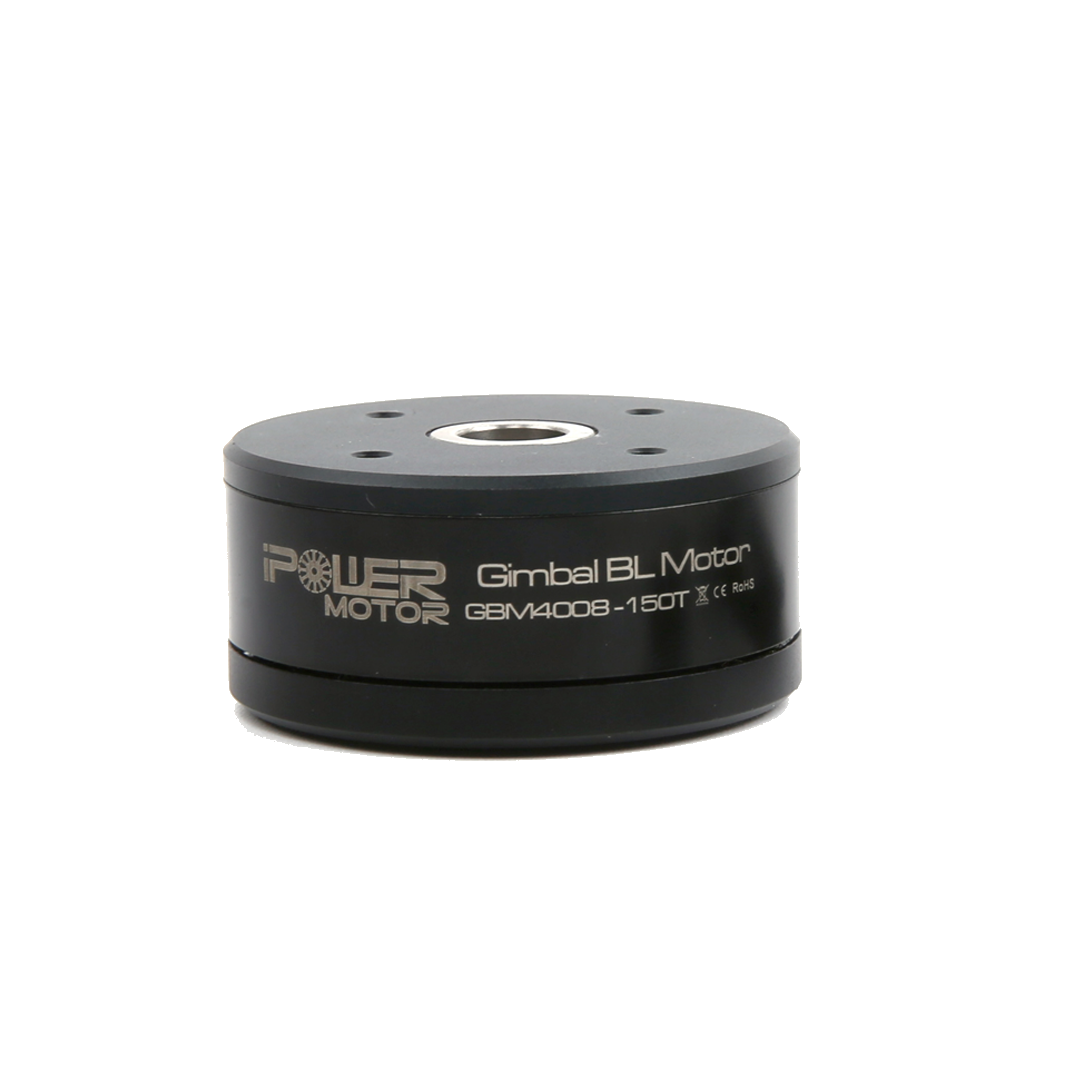
\includegraphics[width=0.5\textwidth,trim={5cm 10cm 5cm 10cm}]{Src/images/GM4008H-1.png}
	\caption{«BLDC Gimbal motor GBM4008H-150T»}
	\label{GBM4008H}
\end{figure}


\begin{table}[H]
	\centering
	\caption{Technical parameters of GBM4008H-150T, GM5208-120T and GM3506 motors}\label{BLDC}
	\begin{adjustbox}{width=\textwidth}

		\arrayrulecolor{black}
		\begin{tabular}{!{\color{black}\vrule}l!{\color{black}\vrule}l!{\color{black}\vrule}l!{\color{black}\vrule}l!{\color{black}\vrule}l!{\color{black}\vrule}l!{\color{black}\vrule}l!{\color{black}\vrule}l!{\color{black}\vrule}l!{\color{black}\vrule}}
			\hline
			Model                                                   & \begin{tabular}[c]{@{}l@{}}Diameter~\\{[}mm]\end{tabular} & \begin{tabular}[c]{@{}l@{}}Height~\\{[}mm]\end{tabular} & \begin{tabular}[c]{@{}l@{}}Weight~\\{[}g]\end{tabular} & Kv & \begin{tabular}[c]{@{}l@{}}Poles \&\\Magnets\end{tabular} & \begin{tabular}[c]{@{}l@{}}Resist.~\\{[}ohms]\end{tabular} & \begin{tabular}[c]{@{}l@{}}Torque~\\{[}kgf-cm]\end{tabular} & \begin{tabular}[c]{@{}l@{}}Max				power~\\{[}W]\end{tabular} \\
			\hline
			\begin{tabular}[c]{@{}l@{}}GBM4008H\\-150T\end{tabular} & 46±0.05                                                                         & 21±0.2                                                                        & 107±0.5                                                                      & 68 & 24N22P                                                    & 6.7                                                                              & 1.2                                                                               & 40                                                                                 \\
			\hline
			\begin{tabular}[c]{@{}l@{}}GM5208\\-120T\end{tabular}   & 63±0.05                                                                         & 22.7±0.2                                                                      & 195±0.5                                                                      & 68 & 24N22P                                                    & 6.7                                                                              & 1.9                                                                               & 40                                                                                 \\
			\hline
			GM3506                                                  & 40±0.05                                                                         & 17.8±0.2                                                                      & 64±0.5                                                                       & 40 & 24N22P                                                    & 5.6                                                                              & 1                                                                                 & 25                                                                                 \\
			\hline
		\end{tabular}
	\end{adjustbox}


	\arrayrulecolor{black}
\end{table}


\subsection{Encoder}

In the design of the control system of the robot arm, the precise determination of the rotation angles of its parts plays an important role. It is also necessary to determine the position of the motor rotor for smoother control. Encoders are commonly used to determine the rotation angle.

One of the most crucial parts is determining the position of each axis link. Precision criteria have special requirements. Based on the technical requirements, it is necessary to ensure a repeatability of 0.02 mm at a distance of 350mm. To achieve this precision, it is required to ensure a minimum axis rotation angle of 0.008185°. The resolution of the absolute encoder should be at least 16 bits, but encoders with such resolution are just beginning to appear and are an expensive solution for this application. It is also important to consider that for vector control, it is necessary to determine the position of the motor rotor to ensure smooth motor startup. The best solution to both problems is to install an encoder on the motor rotor, and due to the gearbox, not only the torque will increase but also the resolving ability of the rotation angle. To ensure acceptable accuracy, it is necessary to use a gearbox with a reduction ratio of at least 11 with a 12-bit encoder resolution. However, it is essential to consider the backlash in all mechanical mechanisms and install harmonic or cycloidal zero-backlash gearboxes \citep{Sensinger2012}.


\begin{figure}[H]
	\centering
	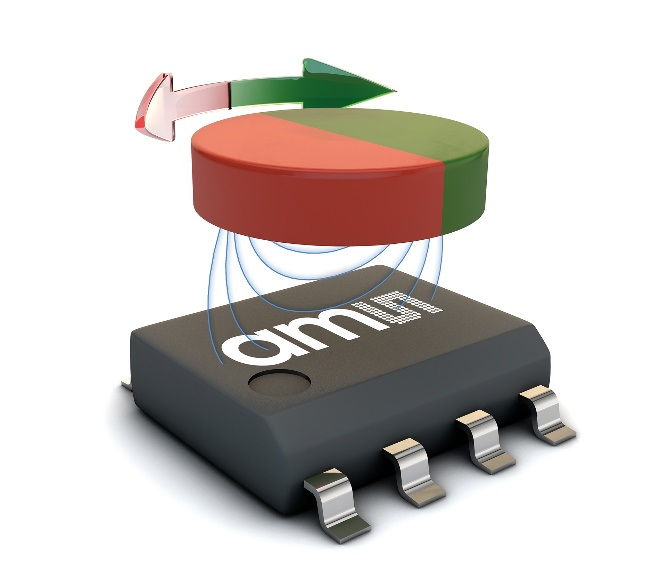
\includegraphics[width=0.5\textwidth]{Src/images/as5600.png}
	\caption{AS5600 axial position detection chip}
	\label{as5600P}
\end{figure}
The AS5600 chip (Fig. \ref{as5600P}) with a digital output from "AMS" was chosen as the encoder. The AS5600 magnetic position sensor is a contactless sensor for determining the absolute rotation angle, providing 12-bit accuracy (Table \ref{as5600T})in measuring angles, ranging from 0 to 360 degrees. 

\begin{table}[H]
	\centering
	\caption{AS5600 axial position chip parameter table}\label{as5600T}
	\begin{tblr}{
		width = \linewidth,
		colspec = {Q[468]Q[445]},
		hlines,
		vlines,
		}
		\textbf{Parameters}       & \textbf{Value} \\
		Resolution				[bit]       & 12             \\
		Output                    & Analog
		out / PWM / I²C                            \\
		Supply				Voltage [V]     & 3-3,6          \\
		Temperature				Range [°C] & -40
		to +125                                    \\
		Package                   & SOIC-8         \\
		Max				current [mA]       & 100            \\
		Sampling				rate [μs]     & 150            \\
		Max
		RPM                       & 20000          \\
		Position				precision [°] & 0.087
	\end{tblr}
\end{table}
AS5600 combines reliability and ease of integration through the use of the I²C digital data transfer interface , making it an excellent choice for continuous and precise monitoring of the motor axis angular position in a robot \citep{ams}.

\subsection{Strategic Control Device}
The Strategic Control Device is essential for solving motion tasks and serves as an interface between the Tactical Control Device and the Intelligent Level Device, thereby providing control over the parameters and the robot itself. The Strategic Control Device must meet the following requirements:
\begin{itemize}
	\item Multitasking capability;
	\item Compact size;
	\item Availability of GPIO;
	\item High computational power;
	\item Ability to use libraries and functions of the operating system;
	\item Low power supply voltage;
	\item Support for wireless communication technologies, IEEE 802.11 or 802.15 specifications.
\end{itemize}

These requirements are met by the single-board mini-computer "Raspberry Pi Zero W 2" (Figure \ref{ZeroP}) from the "Raspberry Pi Foundation". The high computational power of the board (Table \ref{ZeroT}) and the advantages of the "Linux" operating system facilitate the development and execution of complex algorithms and control tasks on the device itself. Moreover, support for a wide range of libraries and access to the 40-pin GPIO connector from the operating system significantly simplifies the development of complex control programs and integration with other systems. Unlike previous "Raspberry Pi Zero" developments, the "Pi Zero 2" modification has a more powerful quad-core "ARM Cortex-A53" processor and a redesigned antenna for better wireless information transmission.

\begin{figure}[H]
	\centering
	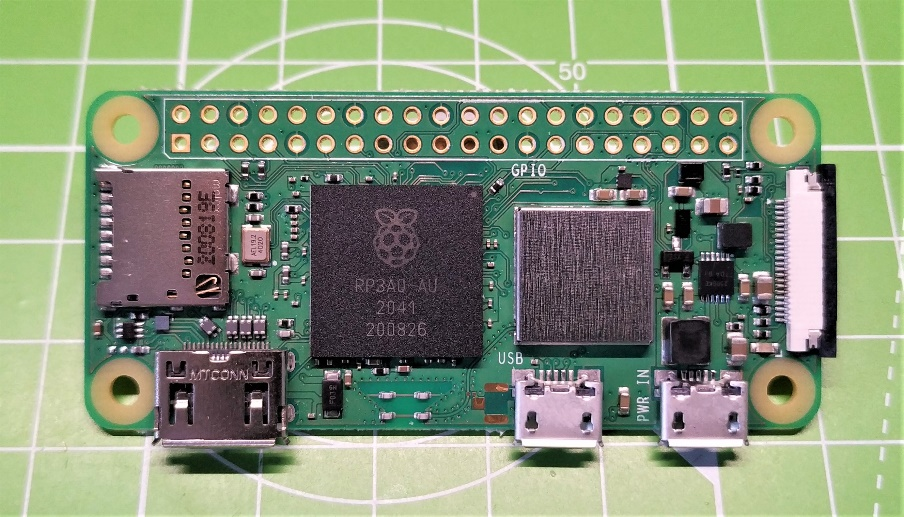
\includegraphics[width=0.6\textwidth]{Src/images/Zero.png}
	\caption{Single-board minicomputer «Raspberry Pi Zero W 2»}
	\label{ZeroP}
\end{figure}




\begin{table}[H]
	\centering
	\caption{Table of parameters of the Raspberry Pi Zero W 2 single-board mini-computer}\label{ZeroT}

	\begin{tblr}{
		width = \linewidth,
		colspec = {Q[180]Q[594]},
		hlines,
		vlines,
		}
		\textbf{Parameters} & \textbf{Value}                      \\
		Processor           & Broadcom
		BCM2710A1, Quad-core Cortex-A53 (ARMv8) 64-bit SoC @ 1GHz \\
		RAM                 & 512MB
		LPDDR2                                                    \\
		Wireless
		Connectivity        & 802.11
		b/g/n wireless LAN, Bluetooth 4.2, BLE                    \\
		Ports               & Mini
		HDMI, USB On-The-Go port, Micro USB power                 \\
		GPIO
		Pins                & 40-pin
		GPIO header                                               \\
		Power
		Requirement         & 5V/2.5A
		DC via micro USB connector or GPIO                        \\
		Size                & 65mm
		x 30mm x 5mm
	\end{tblr}
\end{table}

Based on the requirements to the developed strategic control device, taking into account its specifics, it was decided to use the operating system "Raspberry Pi OS Lite", which is based on the distribution "Debian 12" 32-bit version. The main feature of this distribution is stability, security and wide package support.

\subsection{Tactical and actutor control system controller}

According to the requirements of the developed control system, the control device for tactical and executive devices must be compact; therefore, a microcontroller should be used due to its small size. The microcontroller's tasks include reading and processing data from sensors, facilitating data exchange via the data bus, performing numerical calculations for vector control, solving direct and inverse kinematics problems, and generating PWM signals for the inverter. The minimum requirements for the microcontroller are:
\begin{itemize}
	\item Operating power from 3V;
	\item More than 20 input/output lines;
	\item Ports for working with the CAN bus;
	\item Ports for working with PWM;
	\item Hardware support for the I2C protocol on microcontroller pins;
	\item Presence of an internal ADC;
	\item Presence of a Direct Memory Access (DMA) mechanism.
\end{itemize}

The main problem in choosing a microcontroller was the lack of information related to solving the tasks of the tactical and executive control system. The issue was selecting the best microcontroller model for kinematic tasks. It was impossible to determine which microcontroller, among the most popular on the market, held a leading position. Microcontrollers vary significantly within a single family, and when considering models from different manufacturers, the architecture of each microcontroller is vastly different. It was also necessary to consider the toolchain, the programming tools set, which could also affect performance. Consequently, there was a need to test various types of general-purpose microcontrollers available on the market.
\subsection{Testing microcontrollers}

The conducted testing was necessary to find a suitable microcontroller model. Writing executable programs for each specific microcontroller is a difficult and lengthy process; it is necessary to consider the architecture of the microcontroller and optimize the algorithm for each family. Therefore, synthetic testing was conducted to choose the most suitable microcontroller.

The main selection criterion was the speed of performing specific mathematical operations. High execution speed is necessary to ensure efficient real-time system operation. This is especially important in vector control tasks, where delays in data processing lead to significant losses in accuracy and responsiveness of the entire system as a whole. Upon closer examination of tasks related to kinematics and vector control calculations (in particular, direct and inverse Clarke transformations formulas (\ref{U_a}, \ref{u_b}, \ref{u_c}), inverse Park transformation formulas (\ref{u_park}, \ref{u_park2}), a large number of calculations were discovered \citep{5899203}:
\begin{itemize}
	\item Multiplication and division of floating point numbers;
	\item Calculating trigonometric expressions, sine and cosine functions;

	      \begin{ceqn}
		      \begin{align} \label{u_park}
			      U_\alpha = U_q \sin(\theta)
		      \end{align}
	      \end{ceqn}


	      \begin{ceqn}
		      \begin{align} \label{u_park2}
			      U_\beta = U_q \cos(\theta)
		      \end{align}
	      \end{ceqn}
	\item Square root calculation.
	      \begin{ceqn}
		      \begin{align} \label{U_a}
			      u_a = U_\alpha
		      \end{align}
	      \end{ceqn}

	      \begin{ceqn}
		      \begin{align} \label{u_b}
			      u_b = \frac{-U_\alpha + \sqrt{3}U_\beta}{2}
		      \end{align}
	      \end{ceqn}

	      \begin{ceqn}
		      \begin{align} \label{u_c}
			      u_c = \frac{-U_\alpha - \sqrt{3}U_\beta}{2}
		      \end{align}
	      \end{ceqn}

\end{itemize}



The points mentioned above are complex for computations on the core of any microcontroller and require a large number of processor operations for their calculations. Calculating such expressions will take a significant amount of time, which will negatively affect the performance of the entire control system, as well as the operation of its individual parts \citep{pack2008microcontroller}.

Microcontrollers from manufacturers such as "STMicroelectronics", "Raspberry PI Foundation", and "Espressif Systems" were chosen for the test. The main comparison criterion was the measurement of the time spent on each type of calculation. During the testing, actions related to pausing the main loop of the executable program, such as interrupts, were not used.

\begin{figure}[H]
	\centering
	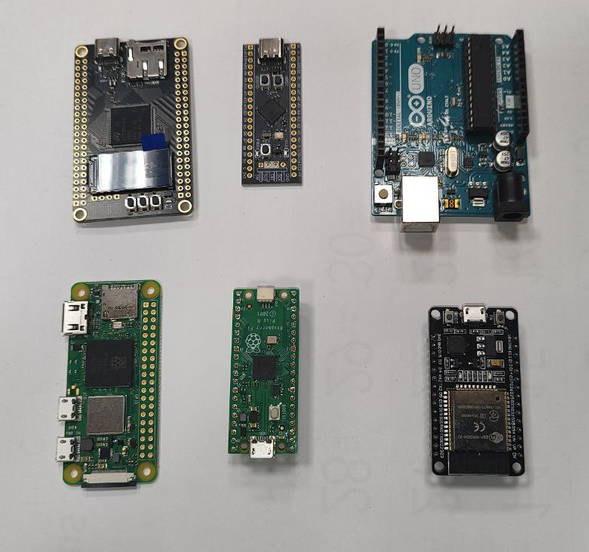
\includegraphics[width=0.4\textwidth]{Src/images/TestDevices.png}
	\caption{Boards that participated in the test}
	\label{Test}
\end{figure}

The \ref{TestT} table lists the microcontrollers used, their clock speeds, and processor model. The boards that participated in the test are shown in the \ref{Test} figure.

% \usepackage{color}n
% \usepackage{tabularray}
\definecolor{DustyGray}{rgb}{0.6,0.6,0.6}
\begin{table}[H]
	\centering
	\caption{List of microcontrollers and their characteristics}\label{TestT}
	\begin{tblr}{
		width = \linewidth,
		colspec = {Q[269]Q[274]Q[146]Q[248]},
		hlines,
		vlines = {Black},
		vline{1} = {-}{DustyGray},
		}
		\textbf{Board} & \textbf{MCU}            & \textbf{Fcpu (Mhz)} & \textbf{CPU}                   \\
		Arduino
		Uno (original) & ATmega328p              & 16                  & AVR                            \\
		NodeMCU-ESP32  & ESP32                   & 240                 & Dual
		Xtensa LX6                                                                                      \\
		NodeMcu
		V3             & ESP8266                 & 160                 & Xtensa
		L106                                                                                            \\
		Raspberry
		Pi Pico        & RP2040				[Arduino IDE] & 133                 & Dual
		Cortex M0+                                                                                      \\
		Raspberry
		Pi Pico        & RP2040				[C++ SDK]     & 133                 & Dual
		Cortex M0+                                                                                      \\
		Raspberry
		Pi Pico        & RP2040				[MicroPython] & 133                 & Dual
		Cortex M0+                                                                                      \\
		STM32
		Nucleo-32      & STM32G431KB             & 170                 & Cortex
		M4                                                                                              \\
		STM32
		Nucleo-32      & STM32G431				[FPU-OFF]  & 133                 & Cortex				M4, \textbf{FPU-OFF}
	\end{tblr}
\end{table}

The essence of the program in the microcontroller was to calculate the time spent using the GPIO port. Before performing the operation, all interrupts are disabled, the microcontroller sets the signal to a high state on the output, the mathematical operation is performed, the microcontroller pin is set to a low state, and the interrupts are restored. Then, using the HMO2024 oscilloscope from the manufacturer "ROHDE \& SCHWARZ", the pulse duration was measured, and the data were recorded in Table \ref{TestTimeT} (the smaller the value, the better). It is worth noting that the calculations took into account the switching time of the GPIO outputs, recorded in the 2nd column of Table \ref{TestTimeT}, and the results are shown in Graph \ref{TestTimeP}.



% \usepackage{color}
% \usepackage{tabularray}

\input{Src/chapters/Colors.tex}

\begin{table}[H]
	\centering
	\caption{Table of measured time to calculate mathematical operations}\label{TestTimeT}

	\begin{adjustbox}{width=\textwidth}

		\begin{tblr}{
				cell{2}{2} = {DeYork},
				cell{2}{3} = {Salomie},
				cell{2}{4} = {Salomie},
				cell{2}{5} = {Salomie1},
				cell{2}{6} = {Salomie2},
				cell{2}{7} = {MacaroniandCheese},
				cell{2}{8} = {MacaroniandCheese1},
				cell{2}{9} = {Salomie2},
				cell{2}{10} = {Carnation},
				cell{3}{2} = {DeYork1},
				cell{3}{3} = {DeYork2},
				cell{3}{4} = {DeYork3},
				cell{3}{5} = {DeYork2},
				cell{3}{6} = {DeYork4},
				cell{3}{7} = {Feijoa},
				cell{3}{8} = {YellowGreen},
				cell{3}{9} = {DeYork5},
				cell{3}{10} = {Salomie3},
				cell{4}{2} = {DeYork6},
				cell{4}{3} = {Feijoa1},
				cell{4}{4} = {Feijoa2},
				cell{4}{5} = {YellowGreen1},
				cell{4}{6} = {Salomie3},
				cell{4}{7} = {Salomie4},
				cell{4}{8} = {Salomie5},
				cell{4}{9} = {Salomie},
				cell{4}{10} = {Chardonnay},
				cell{5}{2} = {DeYork7},
				cell{5}{3} = {YellowGreen2},
				cell{5}{4} = {YellowGreen3},
				cell{5}{5} = {SaharaSand},
				cell{5}{6} = {Salomie3},
				cell{5}{7} = {Salomie6},
				cell{5}{8} = {Salomie7},
				cell{5}{9} = {Salomie3},
				cell{5}{10} = {Grandis},
				cell{6}{2} = {Fern},
				cell{6}{3} = {Feijoa3},
				cell{6}{4} = {Feijoa4},
				cell{6}{5} = {DeYork8},
				cell{6}{6} = {Feijoa5},
				cell{6}{7} = {Salomie8},
				cell{6}{8} = {Salomie8},
				cell{6}{9} = {Feijoa6},
				cell{6}{10} = {Salomie9},
				cell{7}{2} = {Salomie8},
				cell{7}{3} = {Salomie9},
				cell{7}{4} = {Salomie6},
				cell{7}{5} = {Salomie6},
				cell{7}{6} = {Salomie9},
				cell{7}{7} = {Salomie10},
				cell{7}{8} = {Salomie5},
				cell{7}{9} = {Salomie11},
				cell{7}{10} = {Salomie12},
				cell{8}{2} = {Fern},
				cell{8}{3} = {Fern1},
				cell{8}{4} = {Fern1},
				cell{8}{5} = {Fern2},
				cell{8}{6} = {DeYork},
				cell{8}{7} = {DeYork9},
				cell{8}{8} = {Feijoa2},
				cell{8}{9} = {DeYork10},
				cell{8}{10} = {Salomie8},
				cell{9}{2} = {Fern},
				cell{9}{3} = {DeYork6},
				cell{9}{4} = {DeYork11},
				cell{9}{5} = {DeYork12},
				cell{9}{6} = {YellowGreen1},
				cell{9}{7} = {Salomie8},
				cell{9}{8} = {Salomie4},
				cell{9}{9} = {Salomie3},
				cell{9}{10} = {Salomie13},
				hlines,
				vlines,
			}
			MCU                                 & {Time IO\\{[}μs]} & {~a~
			+~ b                                                                                                                                                                                                                                                         \\~[μs]} & {a~ -~ b \\{[}μs]} & {a~
			*~ b\\{[}μs]} & {a~
			/ b\\{[}μs]}  & {sin(a)\\{[}μs]}  & {log(a)\\{[}μs]} & {sqrt(b)\\{[}μs]} & {pow(b, a)\\{[}μs]}                                                 \\
			ATmega328p~                         & 0,144                                   & 9,134                                  & 8,818                                   & 10,141                                    & 31,154 & 104,655 & 155,218 & 31,133 & 328,810 \\
			ESP32                               & 0,312                                   & 0,402                                  & 0,389                                   & 0,399                                     & 0,567  & 0,798   & 1,357   & 0,691  & 3,120   \\
			ESP8266~                            & 0,508                                   & 0,942                                  & 0,959                                   & 1,214                                     & 2,296  & 13,393  & 26,611  & 8,454  & 76,808  \\
			{RP2040~[Arduino IDE]}              & 0,514                                   & 1,477                                  & 1,555                                   & 1,884                                     & 4,233  & 17,052  & 28,012  & 4,090  & 62,245  \\
			{RP2040{[}C++ SDK]}                 & 0,008                                   & 0,750                                  & 0,783                                   & 0,650                                     & 0,819  & 4,634   & 6,610   & 0,709  & 17,288  \\
			{RP2040~[MicroPython]}              & 6,456                                   & 18,412                                 & 17,086                                  & 16,858                                    & 17,499 & 23,491  & 25,253  & 19,688 & 41,450  \\
			STM32G431~                          & 0,005                                   & 0,063                                  & 0,065                                   & 0,056                                     & 0,140  & 0,449   & 0,957   & 0,136  & 5,266   \\
			STM32G431 [FPU-OFF]                 & 0,007                                   & 0,508                                  & 0,529                                   & 0,350                                     & 1,217  & 5,414   & 12,395  & 2,566  & 42,773
		\end{tblr}
	\end{adjustbox}


\end{table}

\definecolor{Fern}{rgb}{0.388,0.745,0.482}

\begin{figure}[H]
	\centering

	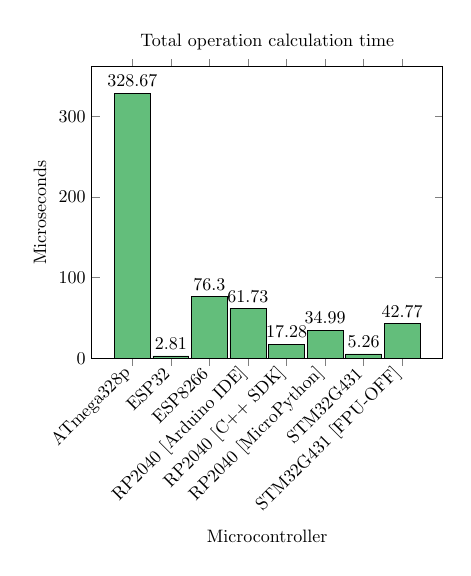
\begin{tikzpicture}[scale=0.65]
		\begin{axis}[
			x tick label style={rotate=45, anchor=east, align=right},
			title=Total operation calculation time,
			xlabel={Microcontroller},
			ylabel={Microseconds},
			ymin=0,
			ybar=5pt, % Adjust the space between bars
			enlarge x limits=0.15, % Add some breathing room between the bars
			bar width=20pt, % Adjust the width of the bars
			symbolic x coords={ATmega328p,ESP32,ESP8266,RP2040 [Arduino IDE],RP2040 [C++ SDK],RP2040 [MicroPython],STM32G431,STM32G431 [FPU-OFF]},
			xtick=data,
			nodes near coords,
			nodes near coords align={vertical},
			]
			\addplot[fill=Fern] coordinates  {
					(ATmega328p,328.667)
					(ESP32,2.808)
					(ESP8266,76.300)
					(RP2040 [Arduino IDE],61.730)
					(RP2040 [C++ SDK],17.280)
					(RP2040 [MicroPython],34.994)
					(STM32G431,5.261)
					(STM32G431 [FPU-OFF],42.766)
				};
		\end{axis}
	\end{tikzpicture}
	\caption{Graph comparing the calculation time of mathematical operations at different MCs}\label{TestTimeP}

\end{figure}


The provided data did not give clear information about the advantages of a specific controller in specific calculations. For further and more convenient analysis, the table was recalculated into the values of thousands of operations per second, kOPS, in Table \ref{TestTimeT2}, using formula (\ref{kops}).


\begin{ceqn}
	\begin{align} \label{kops}
		kOPS= \frac{1000}{T_{cal} - T_{io}}
	\end{align}
\end{ceqn}

% \usepackage{color}
% \usepackage{tabularray}

\begin{table}[H]
	\centering
	\caption{Table comparing thousands of operations per second to calculate mathematical operations of each MCs}\label{TestTimeT2}

	\begin{adjustbox}{width=\textwidth}

		\begin{tblr}{
				cell{2}{2} = {Salmon,r},
				cell{2}{3} = {AtomicTangerine,r},
				cell{2}{4} = {Salmon1,r},
				cell{2}{5} = {Froly,r},
				cell{2}{6} = {Carnation,r},
				cell{2}{7} = {Carnation1,r},
				cell{2}{8} = {Froly,r},
				cell{2}{9} = {Carnation2,r},
				cell{3}{2} = {Feijoa,r},
				cell{3}{3} = {Feijoa1,r},
				cell{3}{4} = {Feijoa2,r},
				cell{3}{5} = {Putty,r},
				cell{3}{6} = {SaharaSand,r},
				cell{3}{7} = {SweetCorn,r},
				cell{3}{8} = {Flax,r},
				cell{3}{9} = {Salomie,r},
				cell{4}{2} = {SaharaSand1,r},
				cell{4}{3} = {SaharaSand2,r},
				cell{4}{4} = {SweetCorn1,r},
				cell{4}{5} = {SweetCorn2,r},
				cell{4}{6} = {Salmon2,r},
				cell{4}{7} = {Froly1,r},
				cell{4}{8} = {AtomicTangerine1,r},
				cell{4}{9} = {Carnation3,r},
				cell{5}{2} = {SweetCorn,r},
				cell{5}{3} = {SweetCorn,r},
				cell{5}{4} = {SweetCorn3,r},
				cell{5}{5} = {Salomie1,r},
				cell{5}{6} = {Salmon3,r},
				cell{5}{7} = {Froly2,r},
				cell{5}{8} = {Salomie2,r},
				cell{5}{9} = {Carnation4,r},
				cell{6}{2} = {SweetCorn1,r},
				cell{6}{3} = {SweetCorn4,r},
				cell{6}{4} = {SaharaSand3,r},
				cell{6}{5} = {SweetCorn4,r},
				cell{6}{6} = {MacaroniandCheese,r},
				cell{6}{7} = {HitPink,r},
				cell{6}{8} = {SweetCorn5,r},
				cell{6}{9} = {Froly3,r},
				cell{7}{2} = {Salmon4,r},
				cell{7}{3} = {Salmon5,r},
				cell{7}{4} = {Salmon6,r},
				cell{7}{5} = {Salmon7,r},
				cell{7}{6} = {Froly3,r},
				cell{7}{7} = {Froly4,r},
				cell{7}{8} = {Salmon8,r},
				cell{7}{9} = {Froly5,r},
				cell{8}{2} = {DeYork,r},
				cell{8}{3} = {DeYork1,r},
				cell{8}{4} = {Fern,r},
				cell{8}{5} = {YellowGreen,r},
				cell{8}{6} = {SaharaSand2,r},
				cell{8}{7} = {SweetCorn,r},
				cell{8}{8} = {YellowGreen1,r},
				cell{8}{9} = {MacaroniandCheese1,r},
				cell{9}{2} = {SaharaSand4,r},
				cell{9}{3} = {SaharaSand4,r},
				cell{9}{4} = {WildRice,r},
				cell{9}{5} = {SweetCorn6,r},
				cell{9}{6} = {MacaroniandCheese2,r},
				cell{9}{7} = {Salmon9,r},
				cell{9}{8} = {Salomie,r},
				cell{9}{9} = {Carnation5,r},
				hlines,
				vlines,
			}
			MCU                  & ~a~
			+~ b                 & a~
			-~ b                 & a~
			*~ b                 & a~
			/ b                  & sin(a)    & log(a)    & sqrt(b)   & pow(b, a)                                           \\
			ATmega328p~          & 111,23    & 115,29    & 100,02    & 32,25     & 9,57     & 6,45     & 32,27    & 3,04   \\
			ESP32                & 11 090,82 & 12 961,74 & 11 549,13 & 3 918,10  & 2 056,26 & 956,62   & 2 641,39 & 356,12 \\
			ESP8266~             & 2 305,87  & 2 217,75  & 1 416,38  & 559,44    & 77,61    & 38,31    & 125,85   & 13,11  \\
			RP2040 [Arduino IDE] & 1 039,35  & 961,04    & 730,02    & 268,92    & 60,47    & 36,37    & 279,68   & 16,20  \\
			RP2040 [C++ SDK]     & 1 347,59  & 1 289,95  & 1 558,30  & 1 232,40  & 216,19   & 151,47   & 1 425,57 & 57,87  \\
			RP2040 [MicroPython] & 83,64     & 94,07     & 96,13     & 90,56     & 58,70    & 53,20    & 75,57    & 28,58  \\
			STM32G431~           & 17 179,17 & 16 702,61 & 19 476,01 & 7 383,89  & 2 253,15 & 1 050,29 & 7 624,36 & 190,09 \\
			STM32G431 [FPU-OFF]  & 1 996,11  & 1 918,50  & 2 917,02  & 826,69    & 184,94   & 80,73    & 390,85   & 23,38
		\end{tblr}
	\end{adjustbox}

\end{table}


The cumulative results of the recalculation of time into the values of thousands of operations per second (kOPS) are presented in Table \ref{TestTimeT2} (higher values are better). 
\definecolor{Salomie10}{rgb}{1,0.89,0.513}
\begin{figure}[H]
	\centering
	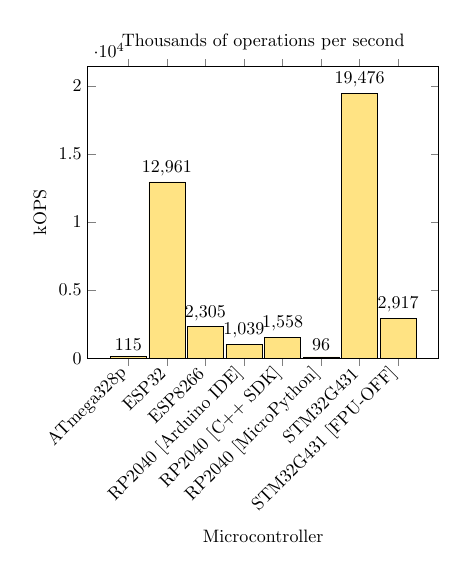
\begin{tikzpicture}[scale=0.65]
		\begin{axis}[
			x tick label style={rotate=45, anchor=east, align=right},
			title=Thousands of operations per second,
			xlabel={Microcontroller},
			ylabel={kOPS},
			ymin=0,
			ybar=5pt, % Adjust the space between bars
			enlarge x limits=0.15, % Add some breathing room between the bars
			bar width=20pt, % Adjust the width of the bars
			symbolic x coords={ATmega328p,ESP32,ESP8266,RP2040 [Arduino IDE],RP2040 [C++ SDK],RP2040 [MicroPython],STM32G431,STM32G431 [FPU-OFF]},
			xtick=data,
			nodes near coords,
			nodes near coords align={vertical},
			]
			\addplot[fill=Salomie10] coordinates  {
					(ATmega328p,115)
					(ESP32,12961)
					(ESP8266,2305)
					(RP2040 [Arduino IDE],1039)
					(RP2040 [C++ SDK],1558)
					(RP2040 [MicroPython],96)
					(STM32G431,19476)
					(STM32G431 [FPU-OFF],2917)
				};
		\end{axis}
	\end{tikzpicture}
	\caption{Graph of maximum values of thousands of operations per second for different MC}\label{TestTimeP2}
\end{figure}
Figure \ref{TestTimeP2} shows the graph of maximum values of thousands of operations per second for each microcontroller. 

In the calculations provided, the microcontrollers performed operations at the maximum possible clock frequency Fcpu, but each microcontroller has a different maximum clock frequency (Table \ref{TestTimeT}). To assess the efficiency of microcontrollers, a calculation of thousands of operations per second per megahertz (\ref{kopsmhs}) was conducted. The graph is shown in Figure \ref{TestTimeP} (higher values are better), and the table with calculations can be found in Appendix 1.
\begin{ceqn}
	\begin{align} \label{kopsmhs}
		kOPS= \frac{K_{OPS}}{Mhz}
	\end{align}
\end{ceqn}
\begin{figure}[H]
	\centering
	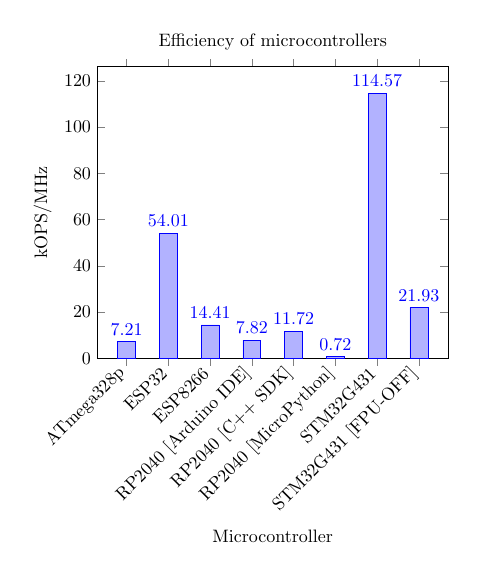
\begin{tikzpicture}[scale=0.65]
		\begin{axis}[
			x tick label style={rotate=45, anchor=east, align=right},
			title=Efficiency of microcontrollers,
			xlabel={Microcontroller},
			ylabel={kOPS/MHz },
			ymin=0,
			ybar, % Controls the space between bars
			symbolic x coords={ATmega328p,ESP32,ESP8266,RP2040 [Arduino IDE],RP2040 [C++ SDK],RP2040 [MicroPython],STM32G431,STM32G431 [FPU-OFF]},
			xtick=data,
			nodes near coords,
			nodes near coords align={vertical},
			]
			\addplot coordinates {(ATmega328p,7.205) (ESP32,54.007) (ESP8266,14.412) (RP2040 [Arduino IDE],7.815) (RP2040 [C++ SDK],11.717) (RP2040 [MicroPython],.723) (STM32G431,114.565) (STM32G431 [FPU-OFF],21.932)};
		\end{axis}
	\end{tikzpicture}
	\caption{ Graph of the values of thousands of operations per second per 1 megahertz of each MCs}\label{TestTimeP3}
\end{figure}


As a result of the tests conducted, several interesting points related to microcontrollers were discovered. As can be seen in Figure 3.4, one RP2040 processor with different sets of development tools yields different results. The test favorites are the ESP32 microcontroller with a Dual Xtensa LX6 processor from the Chinese company "Espressif Systems" and the STM32G431 microcontroller from "STMicroelectronics" with a Cortex M4 processor. The STM chip was more efficient than the ESP32, although the clock frequency of the ESP32 is almost twice as high as that of the STM, but there is no significant increase in mathematical operations. It is worth noting that STM came out on top in terms of time, due to the presence of hardware floating-point operation units (FPU) in the processor.

Additionally, the presence of the "CORDIC" co-processor for hardware acceleration of mathematical operations. As a result, the STM32G431 chip was chosen as the controller for the control system, and Table \ref{MCUData} presents the main characteristics of this chip \citep{stmcordic}.
% \usepackage{tabularray}
\begin{table}[H]
	\centering
	\caption{Table of main characteristics of STM32G431 microcontroller}\label{MCUData}

	\begin{tblr}{
		width = \linewidth,
		colspec = {Q[345]Q[541]},
		hlines,
		vlines,
		}
		\textbf{Parameter} & \textbf{Specification} \\
		Core               & ARM
		Cortex-M4                                   \\
		Operating
		Frequency          & Up
		to 170 MHz                                  \\
		Flash
		Memory             & Up
		to 512 KB                                   \\
		RAM                & Up
		to 128 KB                                   \\
		Digital
		I/Os               & Up
		to 82                                       \\
		Timers             & Multiple,
		including general purpose and advanced      \\
		DAC                & Yes,
		up to 2 channels                            \\
		ADC                & Yes,
		up to 16-bit                                \\
		Interfaces         & I2C,
		SPI, UART, USB, and others                  \\
		Operating
		Voltage            & 2.0
		V to 3.6 V                                  \\
		Temperature
		Range              & -40°C
		to +85°C                                    \\
		CAN
		Bus                & Yes,
		CAN
		2.0 (A, B)                                  \\
		Operational
		Amplifier (Op-amp) & Yes
	\end{tblr}
\end{table}




\subsection{Power Transistors}
Power transistor switches form a three-phase inverter for controlling the electric motor. In this case, the transistor switches are used to amplify the PWM signals coming from the MCU. The type of transistor is N-channel MOSFETs with an induced channel. Such transistors have very low channel resistance (Rds(on)). This means lower power losses when controlling the load, and the component will heat up less, which allows choosing models with smaller dimensions for the same parameter values. The power switches must meet the following requirements:
\begin{itemize}
	\item Operating output voltage is more than 24V;
	\item Operating temperature range -30 to +80;
	\item Transistor type is MOSFET;
	\item Channel type – n;
	\item Small element size;
	\item Type of installation is surface mounting.
\end{itemize}
\begin{figure}[H]
	\centering
	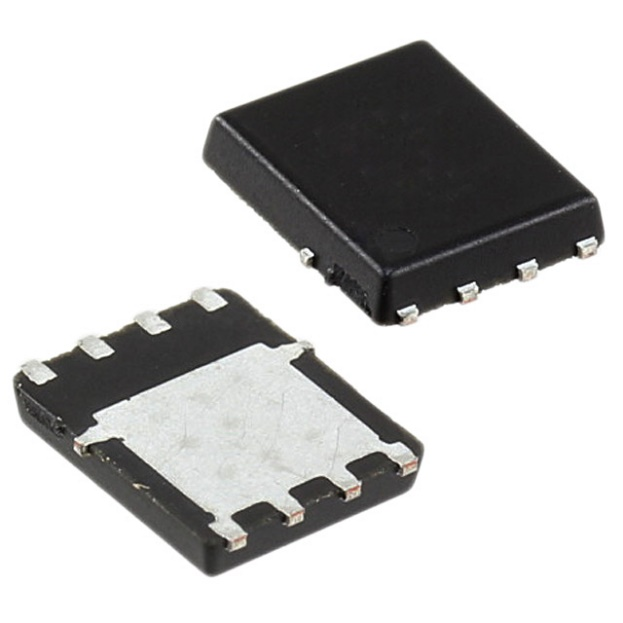
\includegraphics[width=0.5\textwidth]{Src/images/Transistir.png}
	\caption{Transistor «SIR680DP»}
	\label{SIR680DP}
\end{figure}





% \usepackage{color}
% \usepackage{tabularray}
\begin{table}[H]
	\centering
	\caption{Table of main characteristics of transistor SIR680DP}\label{SIR680DPT}

	\begin{tblr}{
		width = \linewidth,
		colspec = {Q[547]Q[374]},
		hlines,
		vlines,
		}
		\textbf{Parameter}  & \textbf{Specification} \\
		Type                & N-Channel              \\
		Drain-Source
		Voltage (VDS)       & 80
		V                                            \\
		Gate-Source
		Voltage (VGS)       & ±
		20 V                                         \\
		Continuous
		Drain Current (ID)  & 100
		A (at TC = 25 °C)                            \\
		Pulsed
		Drain Current (IDM) & 200
		A (for
		100 μs)                                      \\
		Power
		Dissipation (PD)    & 104
		W (at TC = 25 °C)                            \\
		Operating
		Temperature Range   & -55°C
		to +150°C                                    \\
		RDS(on)
		max. at VGS = 10 V  & 0.0024
		Ω                                            \\
		Configuration       & Single                 \\
		Package             & PowerPAK
		SO-8
	\end{tblr}
\end{table}
SIR680DP transistors (Figure \ref{SIR680DP}) from "Vishay Siliconix" were chosen, SIR680DP - 80V/100A n-channel MOSFET. They feature high current density and low open channel resistance (RDS(on)), around 2.4 mΩ, other parameters are in Table \ref{SIR680DPT}, which became the ideal characteristic of a suitable element for use with Pulse Width Modulation (PWM). It is also important to note that the choice of components was dictated by the small size of the "PowerPAK-SO-8" package.
\subsection{Power Transistors Driver}

To facilitate the control of the bridge transistor circuit of the inverter, drivers are used. Their task is to convert a low-power signal taken from the digital output of the MCU into a signal with a higher voltage and power level.

In this implementation of the executive system, general-purpose drivers L6385ED (Figure \ref{L6385ED}) produced by "STMicroelectronics" were used. This chip is a half-bridge driver. One driver can control 2 power transistors of the upper and lower levels. The technical parameters of L6385ED are presented in Table \ref{L6385EDP}.

\begin{figure}[H]
	\centering
	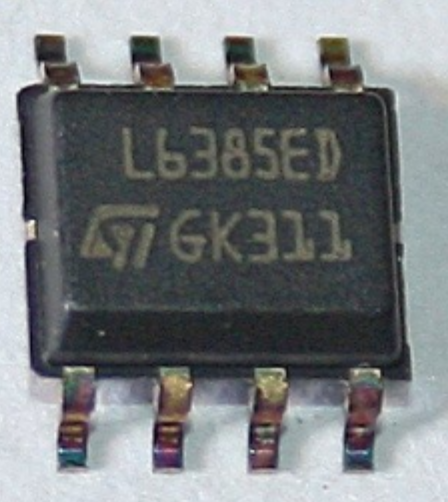
\includegraphics[width=0.3\textwidth]{Src/images/Driver.png}
	\caption{Driver L6385ED}
	\label{L6385ED}
\end{figure}

% \usepackage{color}
% \usepackage{tabularray}
\begin{table}[H]
	\centering
	\caption{Table of L6385ED driver main characteristic}\label{L6385EDP}

	\begin{tblr}{
		width = \linewidth,
		colspec = {Q[324]Q[317]},
		hlines,
		vlines,
		}
		\textbf{Parameter}            & \textbf{Specification} \\
		Maximum
		Operating Voltage             & 580V                   \\
		Supply
		Voltage                       & ±50V/nsec
		(across full temperature range)                        \\
		Driver
		Current Capability (Sourcing) & 400mA                  \\
		Switching
		Time (rise/fall)              & 50/30
		nsec                                                   \\
		Level
		of Input Control Signals      & CMOS/TTL
		Schmitt trigger with hysteresis and pull down          \\
		Under-voltage
		Lockout                       & On
		both lower and upper sections                          \\
		Bootstrap
		Diode                         & Internal
	\end{tblr}
\end{table}

\subsection{Data bus transmitter}
To ensure data transfer between the executive control devices, strategic control, and other devices, it is advisable to use a data bus to reduce the number of connecting conductors. The most suitable data transfer protocol is the CAN bus, which is an industrial standard for industrial networks and has been used multiple times for implementation in manipulator robots \citep{Megalingam2021}.
The main reason for using the CAN bus is its data transfer feature, where data is available to all devices connected to the network. Data transfer to one or several devices simultaneously is possible. Based on this, a synchronization option for all executive devices necessary for timely motion initiation was implemented \citep{stmfdcan}.
Based on the selected microcontroller model in Chapter 3.5 and technical data from Table \ref{TCAN1462DRQ1T}, the hardware support by the microcontroller for the second-generation CAN bus - CAN FD, was identified.

\begin{figure}[H]
	\centering
	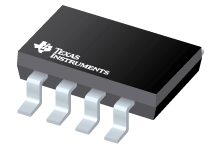
\includegraphics[width=0.3\textwidth]{Src/images/Trans.png}
	\caption{Transceiver TCAN1462DRQ1}
	\label{TCAN1462DRQ1}
\end{figure}





% \usepackage{color}
% \usepackage{tabularray}
\begin{table}[H]
	\centering
	\caption{Table of main characteristics of the TCAN1462DRQ1 transmitter}\label{TCAN1462DRQ1T}

	\begin{tblr}{
		width = \linewidth,
		colspec = {Q[324]Q[317]},
		hlines,
		vlines,
		}
		\textbf{Parameter} & \textbf{Specification} \\
		Package            & SON-8
		(3x3mm)                                     \\
		Operating
		Temperature Range  & -40°C
		to +125°C                                   \\
		Supply
		Voltage Range      & 4.5V
		to 5.5V                                     \\
		Standby
		Current            & Typically
		5μA                                         \\
		Data
		Rate               & Up
		to 5 Mbps                                   \\
		ISO
		11898-2 Compliance & Yes
	\end{tblr}
\end{table}
CAN-FD is the next stage in the development of the classical CAN bus, which provides a higher data transmission rate and a larger amount of transmitted data in one frame, this is possible due to the feature of transmitting field data (CAN data) at a speed multiple of the header transmission rate, which can be up to 8 Mbit/sec.

In order not to limit the possible speed of data transmission on the CAN bus, the TCAN1462DRQ1 transmitter (shown in the figure \ref{TCAN1462DRQ1}) was selected. The transmitter performs signal amplification, line protection in case of CAN bus damage, and adjusts the speed of their transmission.

\subsection{Power converter}
Due to the high consumption of the mini-computer, the consumption reaches up to 2.5A. According to the manufacturer's recommendation it is necessary to use a separate DC to DC converter. The power supply must meet the following requirements:
\begin{itemize}
	\item Input voltage 24V;
	\item DC-DC Converter;
	\item Output voltage 5V,12V;
	\item High output current of 3A or more.
\end{itemize}

The AP64502QSP DC-DC step-down converter chip was selected, shown in Fig. \ref{AP64502QSP}. The advantage of a pulse converter in high efficiency, which does not require heat dissipation, allows for compact voltage and current conversion solutions.
The main advantage of this choice is the ability to convert a high current of 5A (Table \ref{AP64502QSPT}), without the use of external switches and the smaller number of \citep{AP64502Q} elements required to operate this chip.



% \usepackage{color}
% \usepackage{tabularray}
\begin{table}[H]
	\centering
	\caption{Table of main characteristics of the AP64502QSP DC-DC converter}\label{АP64502QSPT}

	\begin{tblr}{
		width = \linewidth,
		colspec = {Q[362]Q[499]},
		hlines,
		vlines,
		}
		\textbf{Parameter}    & \textbf{Specification} \\
		Input
		Voltage Range (VIN)   & 3.8V
		to 40V                                         \\
		Continuous
		Output Current        & 5A                     \\
		Programmable
		Switching Frequency   & 100kHz
		to 2.2MHz                                      \\
		Efficiency
		at Light Load         & Up
		to 85\%                                        \\
		Gate
		Driver Design         & Proprietary,
		for EMI Reduction                              \\
		Frequency
		Spread Spectrum (FSS) & Yes,
		for EMI Reduction                              \\
		Low-Dropout
		(LDO) Mode            & Yes                    \\
		Precision
		Enable Threshold      & For
		UVLO Adjustment                                \\
		Protection
		Features              & UVLO,
		OVP, Peak Current Limit, Thermal Shutdown
	\end{tblr}
\end{table}

\begin{figure}[H]
	\centering
	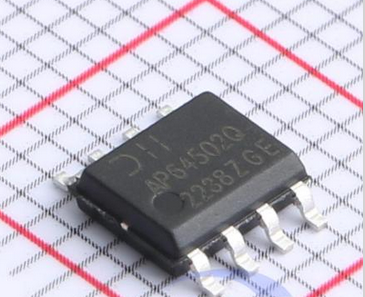
\includegraphics[width=0.3\textwidth]{Src/images/dc-dc.png}
	\caption{DC to DC chip AP64502QSP}
	\label{АP64502QSP}
\end{figure}

\subsection{Functional diagram of the mini robot control system}
The functional diagram of the mini robot arm control system is shown in Fig. \ref{FRobot}.
The main controlling element of the tactical control system is the STM32G431 controlling microcontroller. All the necessary elements are connected to this microcontroller.

Connecting Raspberry Pi Zero W2 (as a strategic device) to the main control element STM32G431 is possible through two interfaces UART, the transfer of information in text form and through SPI, to transfer serialised data of large volumes at high speed. The Raspberry Pi device uses 5 I/O lines:
\begin{itemize}
	\item PA7 (SPI1\_MOSI) \rightarrow GPIO 12 (RPI\_MOSI);
	\item PA6 (SPI1 \_MISO) \rightarrow GPIO 13 (RPI\_MISO);
	\item PA5 (SPI1 \_SCLK) \rightarrow GPIO 14 (RPI\_SCLK);
	\item PA3 (UART2\_RX) \rightarrow RPI (RPI\_TX);
	\item PA2 (UART2\_TX) \rightarrow RPI (RPI\_RX).
\end{itemize}

In order to communicate between the devices of the executive system, a CAN bus transmitter (TCAN1462) is used and the transmitter uses the 2 I/O lines of port B of the STN32G431 microcontroller:
\begin{itemize}
	\item PB9 (FDCAN\_TX) \rightarrow CAN Transceiver (CAN\_TX);
	\item PB8 (FDCAN\_RX) \rightarrow CAN Transceiver (CAN\_RX);
\end{itemize}
For external communication, an RS485 interface transmitter is used, which is connected to the 2 I/O lines of port A.
\begin{itemize}
	\item PA10 (UART2\_TX) \rightarrow RS485 (UART\_TX);
	\item PA9 (UART2\_RX) \rightarrow RS485 (UART\_RX);
\end{itemize}
The robot status is indicated via the display panel and consists of three LEDs of different colours and occupies 3 I/O lines of port B.
\begin{itemize}
	\item PB0 \leftarrow Indication Panel (LED\_YEL);
	\item PB1 \leftarrow Indication Panel (LED\_RED);
	\item PB2 \leftarrow Indication Panel (LED\_GRN);
\end{itemize}
The remaining free I/O lines of the B ports are allocated to digital input and output blocks:
\begin{itemize}
	\item \textbf{Digital inputs:}
	      \begin{itemize}
		      \item[$\circ$] PB11 \leftarrow DI (IN\_1);
		      \item[$\circ$] PB12 \leftarrow DI (IN\_2);
		      \item[$\circ$] PB13 \leftarrow DI (IN\_3);
		      \item[$\circ$] PB14 \leftarrow DI (IN\_4);
		      \item[$\circ$] PB15 \leftarrow DI (IN\_5);
		      \item[$\circ$] PA8 \leftarrow DI (IN\_6);
	      \end{itemize}
	\item \textbf{Digital Outputs:}
	      \begin{itemize}
		      \item[$\circ$] PB7 \rightarrow DO (OUT\_1);
		      \item[$\circ$] PB6 \rightarrow DO (OUT\_2);
		      \item[$\circ$] PB5 \rightarrow DO (OUT\_3);
		      \item[$\circ$] PB4 \rightarrow DO (OUT\_4);
		      \item[$\circ$] PB3 \rightarrow DO (OUT\_5);
		      \item[$\circ$] PA15 \rightarrow DO (OUT\_6);
	      \end{itemize}
\end{itemize}

Connection of all parts of the system is made on the electronic board by soldering the elements. The following connectors will also be used:\begin{itemize}
	\item connectors for operating voltage -- XT30;
	\item CAN bus connectors -- JST 1.25 PH 2;
	\item The pins for the rest of the peripherals -- PBS.
\end{itemize}

XT30 connectors provide a reliable connection and withstand significant electrical loads without loss or risk of fire due to poor contact or overheating.

JST connectors provide easy connection and disconnection, which is convenient for maintenance and system upgrades. They prevent accidental reverse connection, which can be critical to prevent damage to components during installation.

PBS male connectors are suitable for connecting components that do not require high currents and are reusable. Pin connectors provide good contact and ease of mounting on the PCB, which is important for rapid prototyping and system setup.

\begin{figure}[H]
	\begin{adjustbox}{addcode={\begin{minipage}{\width}}{\caption{
							Functional diagram of the mini robot control system
						}\label{FRobot}\end{minipage}},rotate=90,center}
		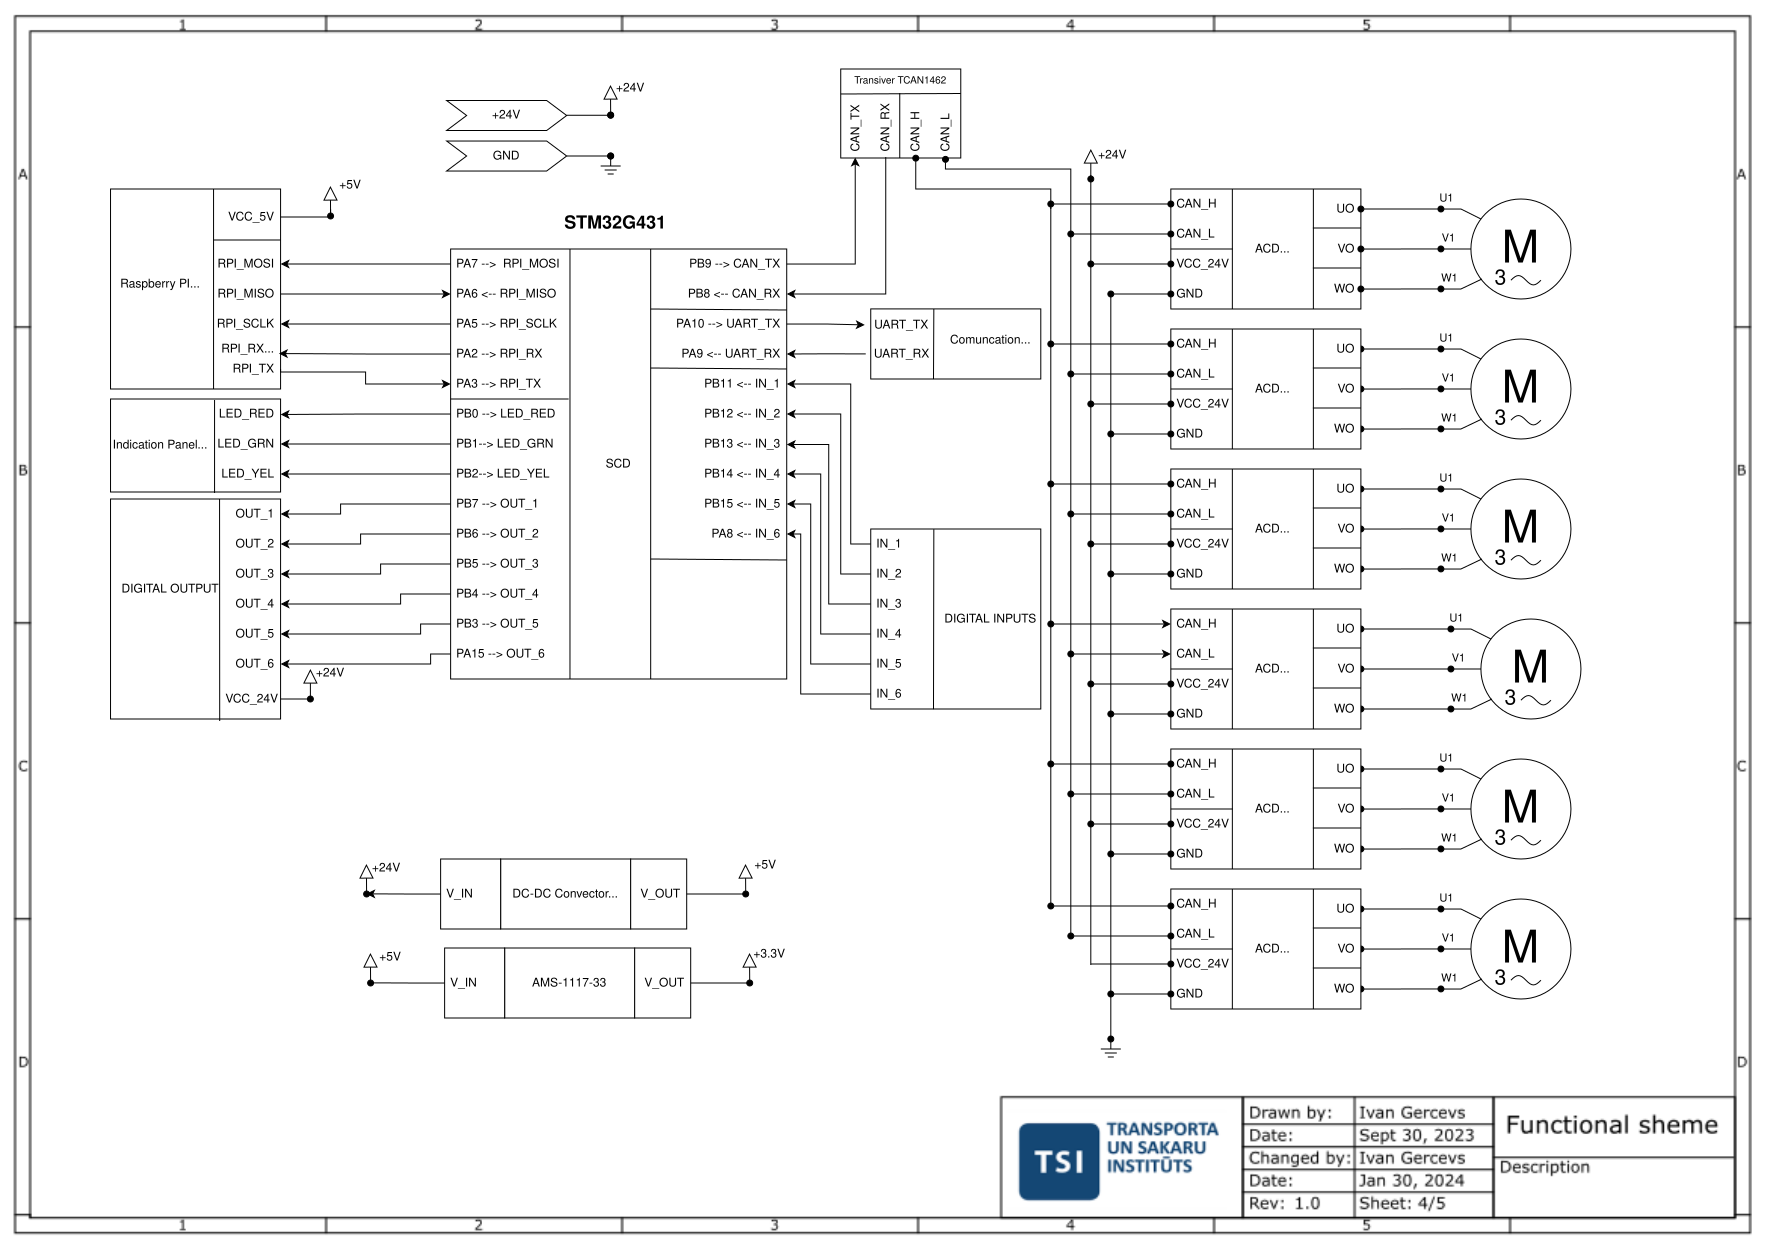
\includegraphics[width=0.85\paperheight]{Src/images/FuncTCD.png}
	\end{adjustbox}
\end{figure}



\subsection{Functional diagram of the actuator control system}
The functional diagram is shown in the figure \ref{FACD}. The main control element of command processing and signal generation, executive control system, is the STM32G431 MCU. Generation of PWM signals is performed by the timer and output by 6 comparison channels, which are output on the lines of port A, C and B:

\begin{itemize}
	\item PB15 \rightarrow HIN1;
	\item PB10 \rightarrow LIN1;
	\item PA12 \rightarrow HIN2;
	\item PB9 \rightarrow LIN2;
	\item PC13 \rightarrow HIN3;
	\item PA8 \rightarrow LIN3;
\end{itemize}
The drivers amplify the signal from the MCU and feed the power key transistors:
\begin{itemize}
	\item HIN1 \rightarrow HGV1;
	\item LIN1 \rightarrow LGV1;
	\item HIN2 \rightarrow HGV2;
	\item LIN2 \rightarrow LGV2;
	\item HIN3 \rightarrow HGV3;
	\item LIN3 \rightarrow LGV3;
\end{itemize}


To measure the torque applied on the motor, there is a measurement of the current mila on each winding of the motor, the voltage drop is measured by feeding signals to the inputs of operational amplifiers which are inbuilt in the microcontroller 6 inputs:

\begin{itemize}
	\item PA1 \leftarrow +VSHUNT\_1;
	\item PA3 \leftarrow -VSHUNT\_1;
	\item PA7 \leftarrow -VSHUNT\_2;
	\item PA5 \leftarrow +VSHUNT\_2;  % Corrected from '-VSHUNT_2' to '+VSHUNT_2' for consistency
	\item PB0 \leftarrow -VSHUNT\_3;
	\item PB2 \leftarrow +VSHUNT\_3;  % Corrected from '-VSHUNT_3' to '+VSHUNT_3' for consistency
\end{itemize}

In order to avoid breakage of the device, two input port lines are provided for connection to the ADC of the microcontroller, one is necessary for temperature measurement, the sensor located near the power transistors, so in case of overheating, the microcontroller takes action to set it to the error state. The second ADC is used to measure the incoming operating voltage, the MC goes into error mode. ADCs are located on the lines of port A and are connected:
\begin{itemize}
	\item PA5 \leftarrow V\_FED; • PA0 \leftarrow V\_BUS;
	
\end{itemize}


\begin{figure}[H]
	\begin{adjustbox}{addcode={\begin{minipage}{\width}}{\caption{
							Functional diagram of the actuator control system
						} \label{FACD}
					\end{minipage}},rotate=90,center}
		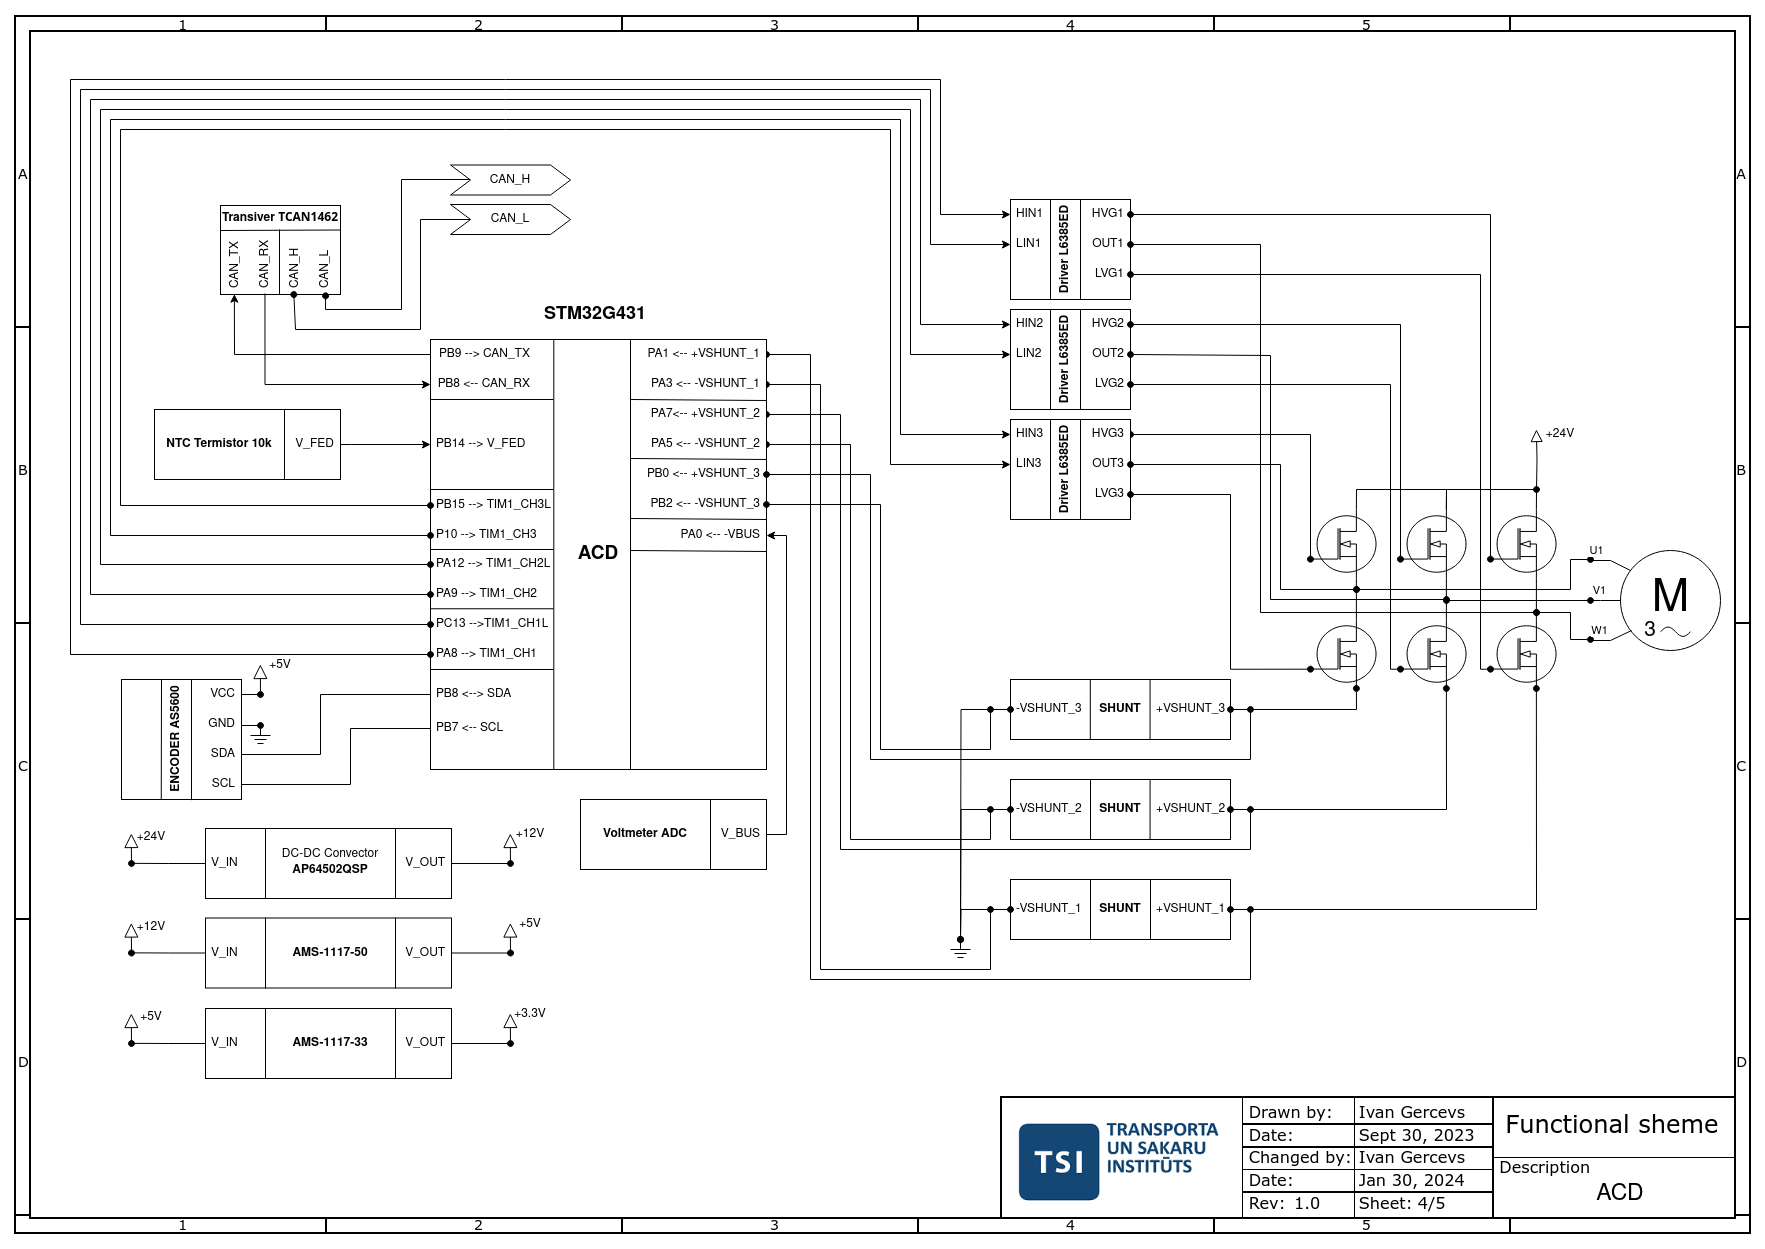
\includegraphics[width=0.85\paperheight]{Src/images/ACD (5).drawio.png}
	\end{adjustbox}
\end{figure}


